\section{Algorithm}

%\subsection{Description}

Punch Out Model Synthesis (POMS) works to progressively resolve chosen
blocks within a larger grid.
Blocks that fully resolve are then saved back into the larger grid.
Should blocks not be able to fully resolve, portions of the grid
are reverted back to an indeterminate state, depending on the mode of failure.


\begin{figure*}[ht]
  \centering
  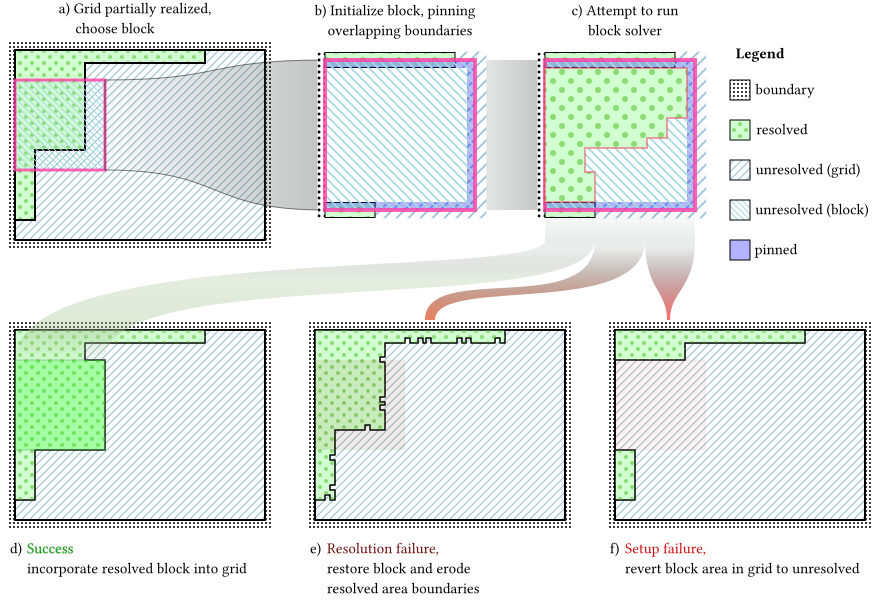
\includegraphics[width=\textwidth]{poms_figalg.png}
  \caption{a) A block is chosen in the partially resolved grid, based on a block choice scheduler
  b) Once the block is chosen, the boundary is pinned if not on the a grid boundary and the center put
  into an indeterminate state. c) The block level solver attempts to find a solution for the block,
  with any pinned boundary restrictions d) If successful, the block is incorporated back into the grid.
  e) If the block solver algorithm failed to resolve, after some maximum iteration count, say, then
  the grid is reverted to its previous state and resolved boundaries are eroded based on an erosion
  choice scheduler. f) If the block solver algorithm failed to start because the block could not be
  put into an arc consistent state given the tiles pinned on the boundary, the block area in the grid is reverted
  to an indeterminate state.}
  \label{fig:alg}
\end{figure*}

%  \Description{A graphical depiction of the Punch Out Model Synthesis algorithm.}

\begin{figure*}[ht]
  \centering
  \includegraphics[width=\textwidth]{pm_slideshow.png}
  \caption{A slideshow of POMS run on the \textit{Pill Mortal} tile set. The block size is 32x32 and the grid size is 64x64 with a block choice policy that chooses block centers uniformly at random from the available unresolved cell locations in the grid. }
  \label{fig:pmrun}
\end{figure*}

%  \Description{Example output of Punch Out Model Synthesis on the Pill Mortal tile set.}

%\subsection{Description}

\begin{algorithm}
  \caption{Punch Out Model Synthesis}
  \label{alg:POMS}
  \begin{algorithmic}
    \State \textbf{Input,Output:} Grid $G$,
    \State \textbf{Input:} Block Choice Scheduler, $BCS$,
    \State \textbf{Input:} Erosion Choice Scheduler, $ECS$,
    \State \textbf{Input:} Block Solver Algorithm, $A$
    \State Set $G$ to a fully indeterminate state
    \While{ $G$ not fully resolved }
      \State Choose block $B$ in $G$ by querying $BCS$
      \State Initialize $B$ to indeterminate state
      \State From $G$, set and pin $B$ edges not on $G$ boundary
      \State Apply initial setup restrictions to $B$
      \State Run $A(B)$ \Comment{Attempt to resolve $B$ with $A$}
      \If{ initial arc consistency is impossible for $B$ }
        \State Set $B$ region to indeterminate state in $G$
      \ElsIf{ $A(B)$ fails to find a full resolution in $B$ }
        \State Erode boundaries in $G$ using $ECS$
      \Else \Comment{success}
        \State Copy fully resolved tiles from $B$ into $G$
      \EndIf

    \EndWhile

  \end{algorithmic}
\end{algorithm}

%Blocks are chosen from a block choice scheduler.
%On successful block resolution, the fully realized block is incorporated back into the grid.
%If the block resolution algorithm fails to initialize the block to an arc consistent state,
%the block area is reverted in the grid.
%Otherwise, if the block solver fails to resolve the block, the boundary of resolved
%regions in the grid is eroded.

POMS retains a copy of the larger grid, keeping either the fully resolved
tile per cell or an indicator that the cell is in an indeterminate state.
Each round consists of choosing a block from some block choice scheduler 
and doing full block level resolution from some underlying block level algorithm.
%such as Wave Function Collapse (WFC) or 
%Breakout Model Synthesis (BMS) \cite{Hoetzlein_2023}.
In this paper, we only consider Breakout Model Synthesis (BMS) \cite{Hoetzlein_2023}
for the underlying block level resolution algorithm.


Each block chosen has its boundary pinned to the values as they appear in the grid,
except if the block boundary falls on the grid boundary.
Here, \textit{pinning} means setting a cell's tile domain to a certain set of values
and not allowing any constraint propagation to be performed on the cell.
The pinned cell's tile domain can affect a neighboring cell tile but is otherwise not
considered for constraint propagation.
For the block boundary pinning, the block boundary cell's tile domain is restricted to a single tile value,
taken from the tile at the grid cell.
Pinning ensures that the block can integrate into the larger grid by guaranteeing
the boundary conditions of the block match the related regions in the grid.

If the block and grid share a boundary, the tiles at the cell boundaries are not
pinned but are subject to boundary conditions.
Here, we only consider boundary conditions where a fixed tile is used when neighboring
constraints would fall out of grid bounds.

Block regions are chosen by a \textit{Block Choice Scheduler} (BCS) as referenced in Algorithm \ref{alg:POMS}.
From our experimentation, the BCS is problem specific and will be discussed later (Section 4).

Once a block is chosen, the block is initialized by adding the full tile domain of tile values
to every block cell, applying setup restrictions and then running an initial constraint propagation
that attempts to put the block in an arc consistent state.
The setup restrictions only allow for tiles to be added, removed
or pinned on an individual cell.
Once setup restrictions are imposed, an attempt is made to run the constraint propagation and
put the block in an arc consistent state.

%When first choosing a block, an initial attempt is made to put it into an arc consistent state.
If the block is successfully put in an arc consistent state, the block level resolution algorithm proceeds and attempts to find a fully realized block.
If a fully realized block is found, it's put back into the grid and the algorithm
continues on by choosing another block until the grid is fully realized.

Should the initial attempt to put the block choice into an arc consistent state fail,
the block region is reverted to an indeterminate state in the grid.
The motivation for reverting the whole block region, as opposed to just relying on erosion,
is that if a block cannot be put into an arc consistent state, subject to its pinned
boundary values, there might be a strong contradiction that requires an aggressive
back-off strategy.

If the initial block level arc consistency attempt succeeded but the block level resolution
algorithm failed to find a fully realized block,
boundary tiles of fully resolved regions are probabilistically reverted to an indeterminate state.
The process of probabilistically reverting boundary cell locations to indeterminate states is called \textit{erosion},
with the \textit{probability of erosion} being a tunable parameter that sets the probability that a cell located on a resolved boundary
is reverted.

Algorithm \ref{alg:POMS} gives pseudo code for the Punch Out Model Synthesis (POMS) algorithm.
Figure \ref{fig:alg} gives an overview of the POMS algorithm, highlighting
a single step.
Figure \ref{fig:pmrun} shows a slideshow of POMS being run on the \textit{Pill Mortal}
tile set for a 64x64 grid size with 32x32 block size.

The probability of erosion is managed by the \textit{Erosion Choice Scheduler} (ECS) as referenced in Algorithm \ref{alg:POMS}.
We have found that a good choice for ECS is to increase the erosion probability by the number of failed attempts, allowing
for a more aggressive erosion strategy should block resolution become increasingly difficult.
Without the erosion, block level solvers could be doomed
to perpetually attempt resolution on blocks with identical initial state.
The erosion provides a backtracking mechanism, allowing for a change in initial state
of chosen blocks and potentially removing contradictions on resolved regions in the grid.

Maximum iteration counts can be added so that POMS or the underlying block level resolution
algorithm ($A$) don't loop forever.
The iteration counts and other checks in Algorithm \ref{alg:POMS} have been omitted for brevity.

%The block choice scheduling strategy and the erosion strategy can be tuned to be problem
%specific.
%In practice, we have found that a block choice policy of a growing resolved region, such
%as sweeping from one side to another or working from the middle out, works
%well in many instances.
%We have found a good choice of erosion strategy is to erode after every other full resolution
%failure and with a decreasing probability as a function of resolution progress.

Since the grid only keeps one value per cell and full constraint propagation is done
on a block level, only a block level's worth of data need be kept in active memory.
Full constraint propagation is done on an individual block level but the block size can be
chosen to be much smaller than the grid, allowing block sizes to be tuned as resources allow.

%If it is too restrictive to fix a tile value that neighbors grid edge boundaries,
%a grid realization can be done by pinning the full tile domain ($D$) of the tile set on a one cell boundary on each edge of the grid.
%The pinning ensures that no tile will ever be removed from the one cell edge boundary and
%creates an effective ``wild card'' option that does not further restrict interior cell tile choice options.
%Since the edge pinning falls under the setup restriction step, this can be done from specifying the initial setup restriction
%conditions and does not require further modification of the underlying POMS algorithm.

The indeterminate state of the larger grid also imposes minimal assumptions for setup,
as there is no need for a fully realized initial state.
Further, the lax assumptions on initial state allow for more freedom
in choosing initial restrictions.


